\documentclass[11pt]{article}

\usepackage{amsmath,amssymb}
\usepackage[usenames,dvipsnames,svgnames,table]{xcolor}
\usepackage[colorlinks=true,citecolor=blue]{hyperref}
\usepackage{natbib}
\usepackage{graphicx}
\usepackage{setspace}
\usepackage{framed}

% \doublespacing

\begin{document}

%%%%%%%%%
\title{SpeciesNetwork Tutorial \\
\large Inferring Species Networks from Multilocus Data}
\author{Chi Zhang \\
E-mail: zhangchi@ivpp.ac.cn}
\maketitle

%%%%%%%%%
\section*{Introduction}

This tutorial describes a full Bayesian framework for species network inference studying reticulate evolution. The statistical methodology is described in \citet{Zhang:2017gq}.
You will need the following software at your disposal:
\begin{itemize}
\item {\bf BEAST} --- this package contains the BEAST program, BEAUti, and other utility programs. This tutorial is written for BEAST v2.4.7 or higher \citep[\url{http://beast2.org},][]{Bouckaert:2014iz}.
\item {\bf Tracer} --- this program is used to explore the output of BEAST (and other Bayesian MCMC programs). It summarizes graphically and quantitively the distributions of continuous parameters and provides diagnostic information for the particular MCMC chain (\url{http://tree.bio.ed.ac.uk/software/tracer}).
\item {\bf IcyTree} --- this is a web application for visualizing phylogenies, including phylogenetic networks \citep[\url{icytree.org};][]{Vaughan:2017fu}.
\end{itemize}

%%%%%%%%%
\section*{The Data}

The multilocus sequence alignment used to illustrate the analysis is simulated under JC69 substitution model \citep{Jukes:1969wx} with strict molecular clock and no rate variation across loci, on the gene trees simulated under the species network shown in Figure \ref{fig_spnetwork} \citep[see also][]{Zhang:2017gq}. There are 2 sequences from species $A$, 4 from $B$ and 2 from $C$ for each of the 10 loci. The sequence length is 200bp per locus. The NEXUS file called {\bf 10loci.nex} is included with this tutorial.

\begin{figure}[h]
\center
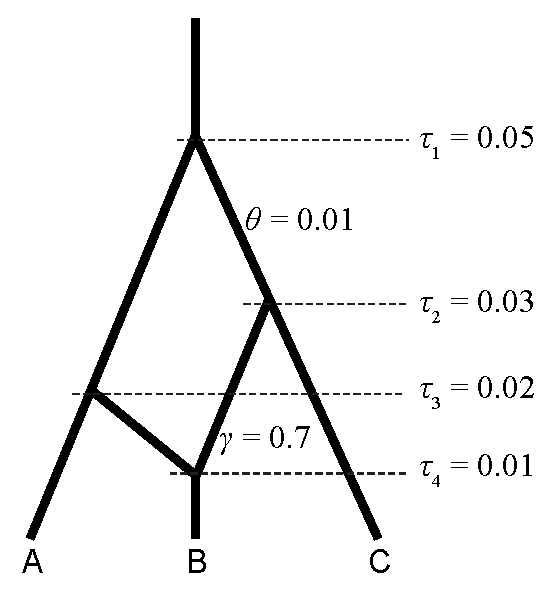
\includegraphics[width=0.4\textwidth]{figs/fig1_spnetwork}
\caption{Species network used to simulate the data}
\label{fig_spnetwork}
\end{figure}

\section*{Set up BEAUti}

The first step in the analysis will be to convert the NEXUS files into a BEAST XML input file. This is done using the program {\bf BEAUti} included in the BEAST package. This is a user-friendly program for setting the evolutionary model and options for the MCMC analysis. The second step will be to actually run BEAST using the XML input file that contains the data, model and MCMC chain settings. The final step will be to explore the output of BEAST in order to diagnose problems and to summarize the results.

SpeciesNetwork uses a non-standard template to generate the XML, so the first thing to do is to change the template. Choose the {\bf File / Template / SpeciesNetwork} item (Fig. \ref{fig_template}). If you do not see this template in the menu, make sure the SpeciesNetwork plugin is installed correctly.
Keep in mind that when changing a template, BEAUti deletes all previously imported data and starts with a clean template. So, if you already loaded some data, a warning message will pop up indicating that this data will be lost if you switch templates.

\begin{figure}[h]
\center
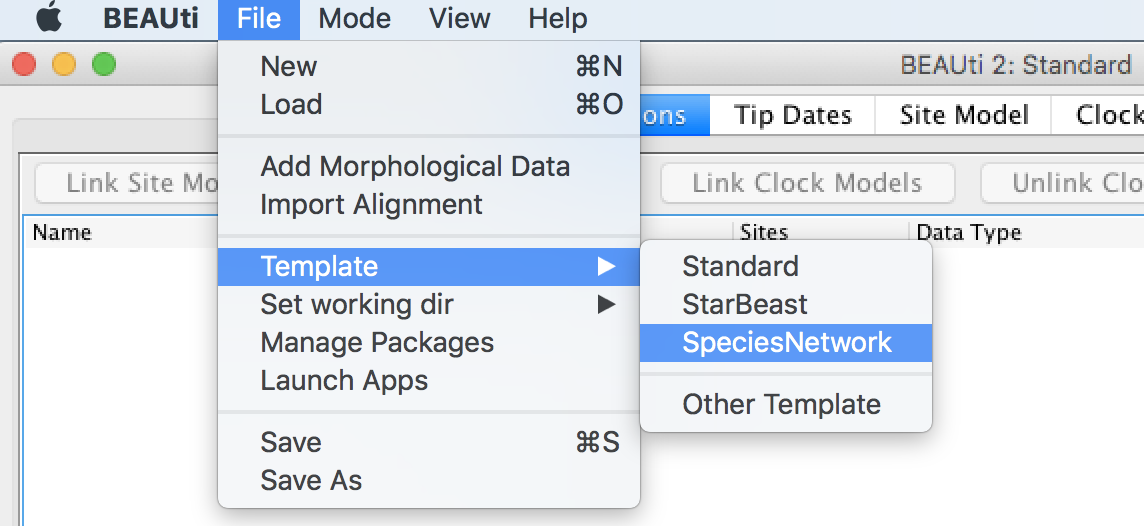
\includegraphics[width=0.7\textwidth]{figs/fig2_template}
\caption{Select a new template in BEAUti, then import the alignment}
\label{fig_template}
\end{figure}

\section*{Load the NEXUS file}

To import the sequence alignment into BEAUti, use the {\bf Import Alignment} option from the {\bf File} menu (Fig. \ref{fig_template}) and select 10loci.nex. Once loaded, the 10 loci are displayed in the Partitions panel. You can double click any locus (partition) to show its detail.

For multilocus analyses, BEAST can link or unlink substitution, clock, and tree models across loci by clicking buttons at the top of the Partitions panel. The default is unlinking all models.
Since the species are contemporary and the implementation can not incorporate node calibrations (except for the origin), plus that the purpose here is not to explore evolutionary rate variation across gene tree lineages through relaxed clock models, we link the clock models for all loci and rename the label to {\bf allloci} (Fig. \ref{fig_partition}). The clock rate will later be fixed to 1.0 in the Clock Model panel. The evolutionary rate variation across different gene loci will be modeled using gene-rate multipliers and set in the Site Model panel (see below).
You should only unlink the tree models across loci that are actually genetically unlinked. For example, in most organisms all the mitochondrial genes are effectively linked due to a lack of recombination and they should be set up to use the same tree model.

\begin{figure}[h]
\center
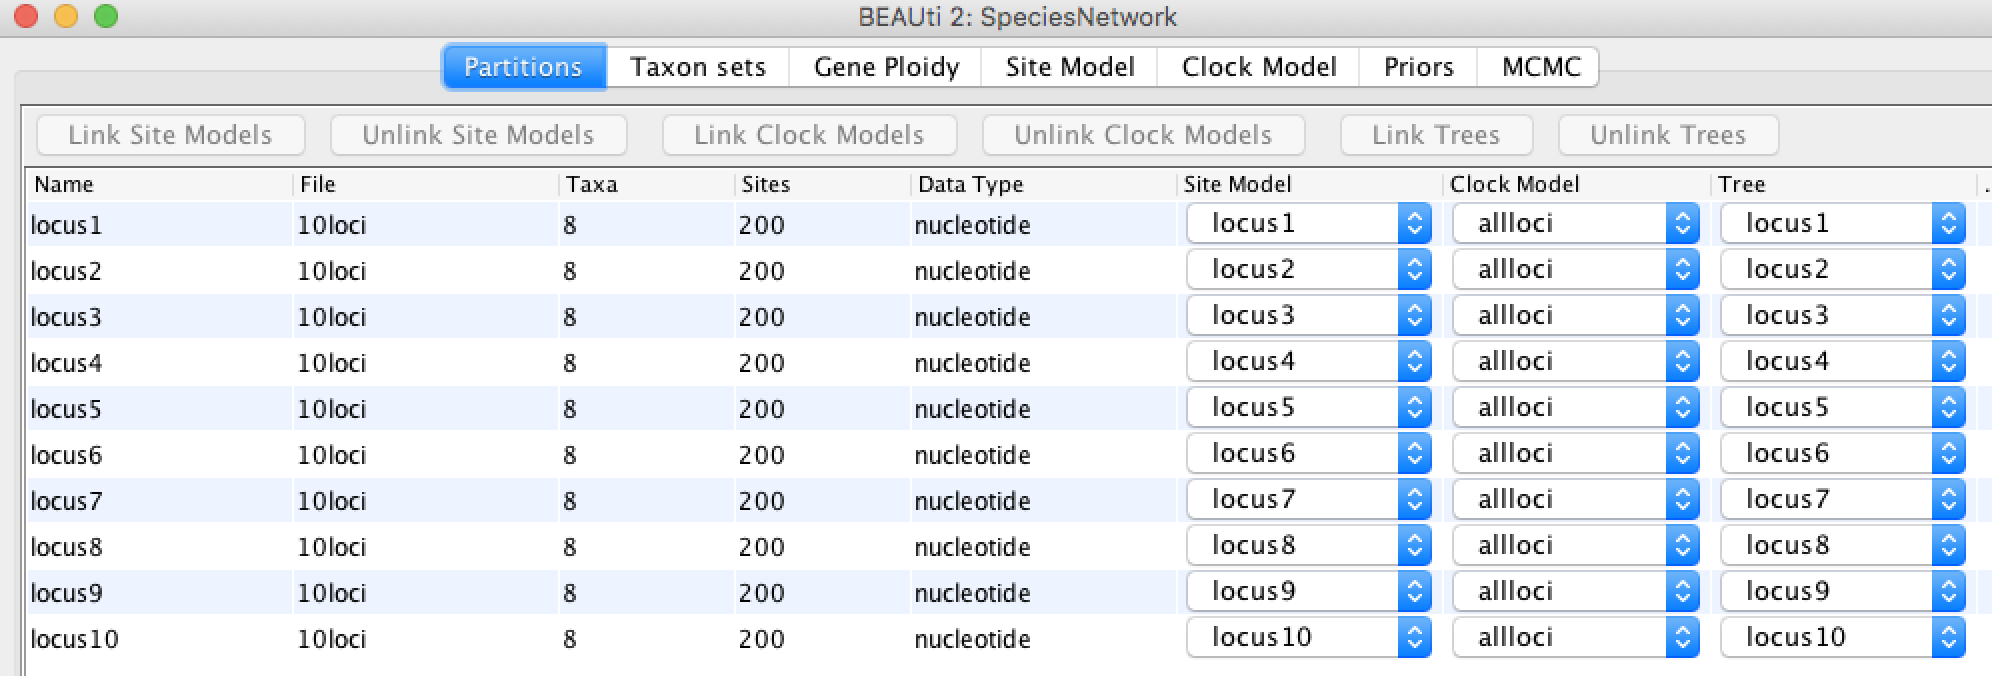
\includegraphics[width=1.0\textwidth]{figs/fig3_partition}
\caption{Partition panel after loading the alignment}
\label{fig_partition}
\end{figure}

\section*{Assign taxa to species}
Each taxon should be assigned to a species, and this mapping is fixed during the analysis. Typically, the species name is already embedded inside the taxon name and should be easily extracted. If the default guess by BEAUti is not satisfactory, press the {\bf Guess} button at the bottom and a dialog will show up where you can choose from several ways to try to detect the species names. Otherwise the names can be filled in manually (Fig. \ref{fig_mapping}).

\begin{figure}[h]
\center
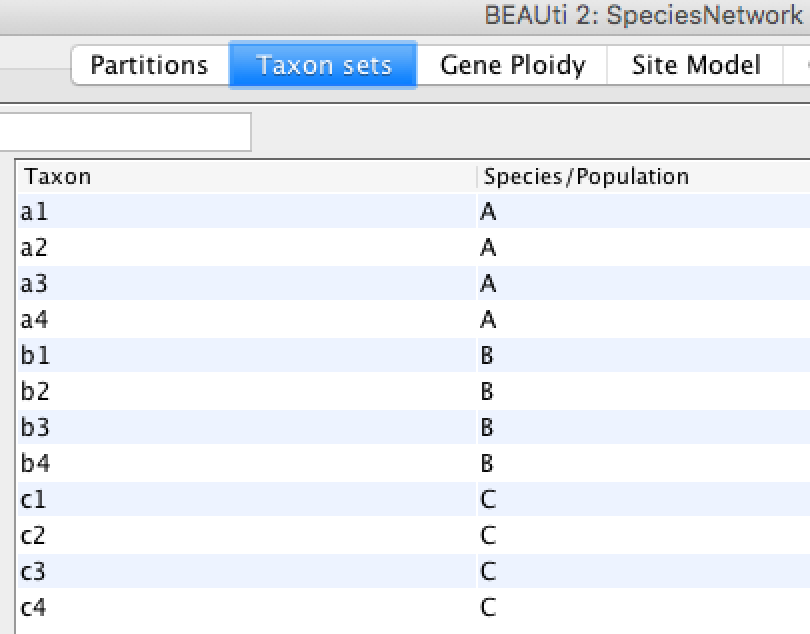
\includegraphics[width=0.6\textwidth]{figs/fig4_mapping}
\caption{Assigned taxa to species}
\label{fig_mapping}
\end{figure}

\section*{Set gene ploidy}

Ploidy should be based on the mode of inheritance for each gene. By convention, nuclear genes in diploids are given a ploidy of 2.0. Because mitochondrial and Y chromosome genes are haploid even in otherwise diploid organisms, and also inherited only through the mother or the father respectively, their effective population size is only one quarter that of nuclear genes. Therefore if nuclear gene ploidy is set to 2.0, mitochondrial or Y chromosome gene ploidy should be set to 0.5. All genes in the simulation are assumed from nuclear loci and their ploidy should be left at the default value of 2.0 in the Gene Ploidy panel.

\section*{Set up substitution and clock models}

The next thing to do is to set up the substitution and clock models.
Although the true substitution model in the simulation is JC69 which is the default in the Site Model panel, we select the {\bf HKY} model \citep{Hasegawa:1985ww} that will fit better for real data. The frequencies are set to {\bf empirical} so that only the $\kappa$ parameter is {\bf estimated} (Fig. \ref{fig_sitemodel}).
To account for evolutionary rate variation across loci with mean 1.0, tick {\bf estimate} at {\bf Substitution Rate} (Fig. \ref{fig_sitemodel}) to use the gene-rate multipliers.

\begin{figure}[h]
\center
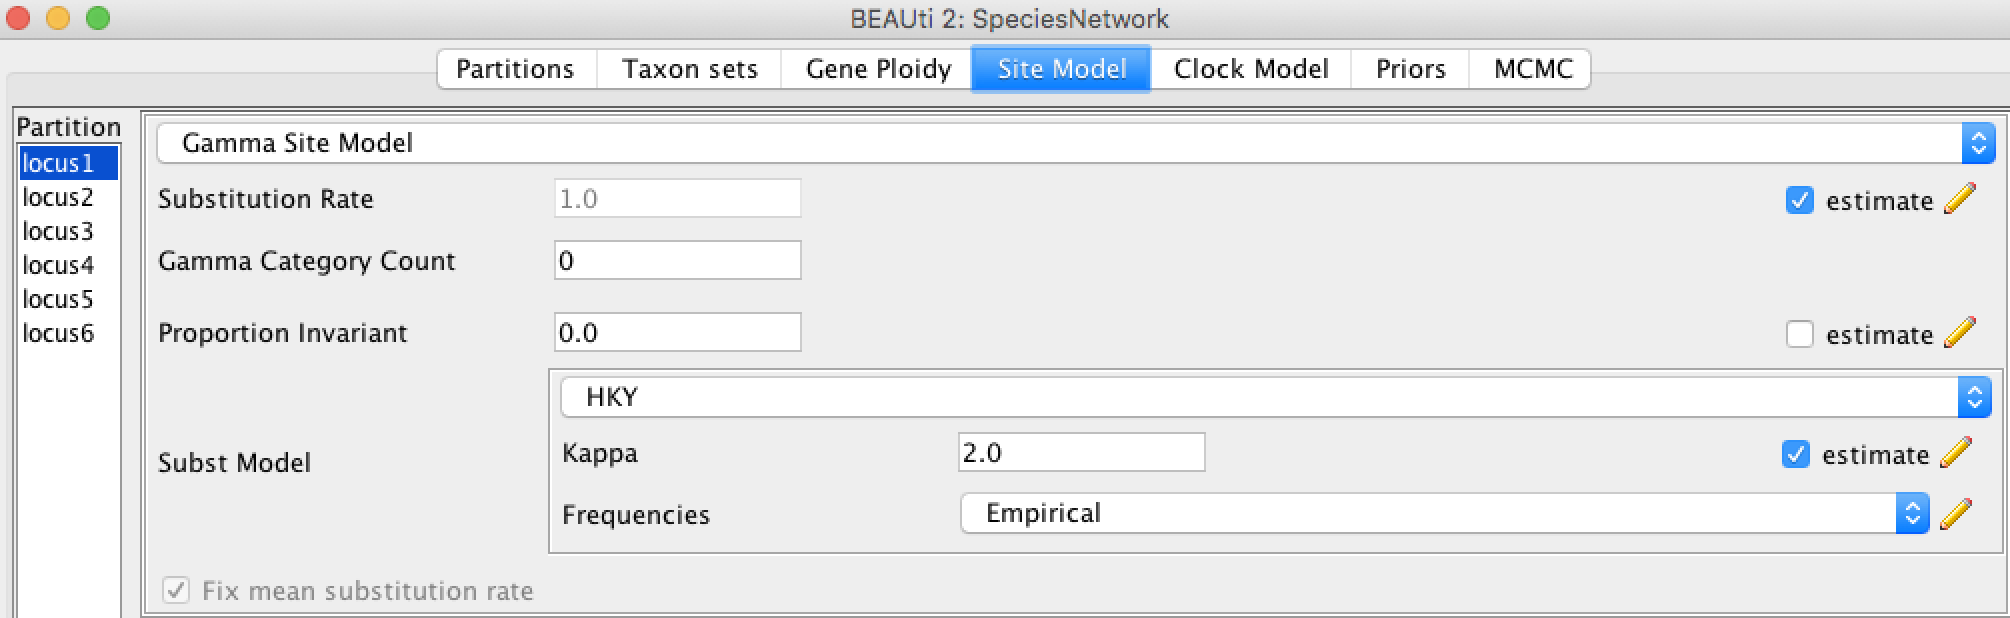
\includegraphics[width=1.0\textwidth]{figs/fig5_sitemodel}
\caption{Setting up substitution models}
\label{fig_sitemodel}
\end{figure}

Uncheck {\bf estimate} in the Clock Model panel to fix the clock rate to 1.0 for all loci.
\begin{figure}[h]
\center
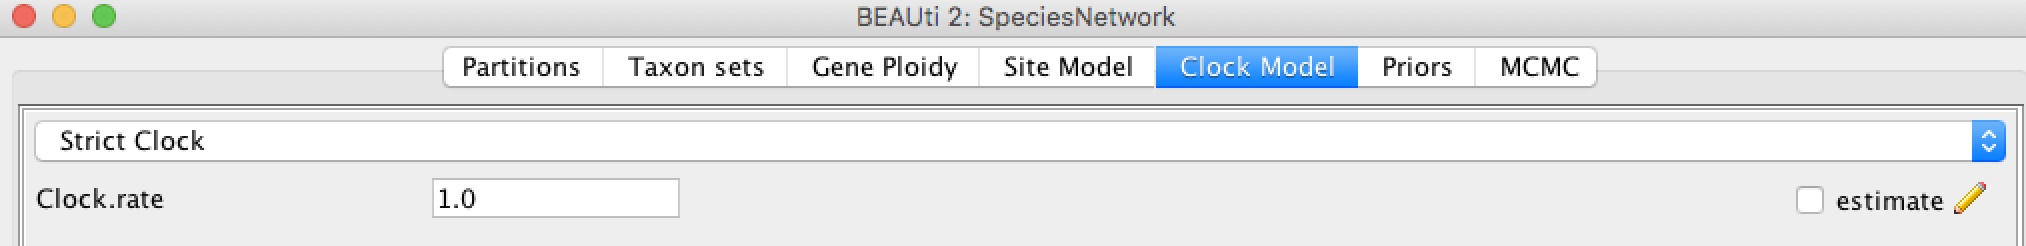
\includegraphics[width=1.0\textwidth]{figs/fig6_clockmodel}
\caption{Setting up clock models}
\label{fig_clockmodel}
\end{figure}

\section*{Priors}

The {\bf Priors} panel allows priors for each parameter in the model to be specified. The default priors that BEAST sets for the parameters would allow the analysis to work. However, some of these are inappropriate for this analysis. Therefore change the priors as follows:



%%%%%%%%%  REFERENCE    %%%%%%%%%%%%%%%
\bibliographystyle{mbe}
\bibliography{refs}

\end{document}
